\chapter{Track Classification NN}\label{chap:track_classification_mva}

This chapter details work on implementing a neural network (NN) to predict the truth origin of reconstructed tracks.
An introduction to the formalism of machine learning is given in \cref{sec:ml_background}.
In \cref{sec:track_labelling}, the truth origin label is defined, and in \cref{sec:fake_track_mva} these labels are used to train a machine learning model that can effectively discriminate between good and fake tracks.
Several studies motivated this work by demonstrating that at high \pt, the performance of the low-level \btagging algorithms was degraded by the presence of large numbers of poorly reconstructed or fake tracks.
If a separate algorithm could be trained to detect fake tracks, these could be removed before their input to the \btagging algorithms with the aim of improving performance.
The identification of fake tracks could also be used to improve the reconstruction of other physics objects which rely on tracking information, for example $\tau$ leptons or track-jets.


\section{Machine Learning Background}\label{sec:ml_background}

Over the past few decades, machine learning (ML) techniques have become increasingly prevalent in High Energy Physics experiments due the increased volumes of high-dimensional data and improvements in the field of deep learning.
Machine learning is the process by which a computer program uses data to infer suitable parameters for a predictive model.
This is opposed to providing explicit instructions on how to perform a task.
A subfield known as \textit{supervised learning} is used in this work, and consists of exposing a model to a large number of labelled examples in order to extract relationships between the input data and their labels.
These relationships are often complex, and explicitly programmed rules can fail to fully capture the relationships between inputs and outputs.

%The field of machine learning aims to design computer programs which, rather than being programmed explicitly with instructions on how to perform a specific task, instead learn from a set of labelled training examples $S_i$ how to perform the task for themselves, essentially replacing the need to manually design a program to perform a specific task.
%In this section a subset of machine learning techniques called supervised learning is described.

In the simplest case, a set of $m$ labelled training examples $S = \{ (x_1, y_1) , \ldots , (x_m, y_m) \}$ is collected.
Each element $(x_i, y_i)$ consists of a input vector $x_i  \in \mathbb{R}^{\textnormal{input}}$, and the corresponding label $y_i$.
In classification problems, these labels are integer \textit{class labels} $y_i \in \{0,\ldots,N-1\}$, where $N$ is the number of classes, which specify which of a pre-determined set of categorical classes the training example belongs to.
The rest of the discussion in this chapter is limited to binary classification problems ($N = 2$).
The two classes are often referred to as signal ($y_i = 1$) and background ($y_i = 0$), which need to be separated.
Collecting sufficient and suitable data is one of the primary challenges of machine learning, as such data is not always readily available.
Fortunately, sophisticated tools to simulate particle collisions have already been developed by the scientific community \cite{Boos:2001cv,leshouchesstandardisation}.
These tools play a key role in generating a suitably large amount of labelled data which is used to train algorithms.
More detail on the input datasets can be found in \cref{sec:track_classifier_datasets}.

After obtaining suitable training data, the next step is to define a model.
Given an input domain $\mathbb{R}^{\textnormal{input}}$ and an output domain $(0, 1)$, the model
$f_\theta: \mathbb{R}^{\textnormal{input}} \to (0, 1)$ is a parameterised functional mapping from input space to output space.
Given an input example $x_i$ and a set of parameters $\theta$, the model outputs a prediction $\hat{y}_i \in (0, 1)$ for the true label $y_i$, as in
%
\begin{equation}
    f_\theta(x_i) = \hat{y}_i .
\end{equation}
%
The output $\hat{y}_i$ is in the interval $(0, 1)$ so as to be interpreted as the probability that the input example $x_i$ belongs to the signal class.
The parameters $\theta$ of the model are randomly initialised, and the model is designed to be expressive enough to correctly map the inputs $x_i$ to the outputs $y_i$ given a reasonable optimisation of the parameters.
To perform this optimisation, the model is then trained, which amounts to showing the model a series of labelled training examples and modifying the parameters of the model based on its ability to correctly predict the labels.


\subsection{Neural Networks}\label{sec:neural_nets}

Neural networks (NNs) are a common choice for the machine learning model $f$ since they have the ability to approximate any function \cite{HORNIK1989359} and are easy to train via backpropagation \cite{rumelhart1986learning}.

\subsubsection{Artificial Neurons}

The basic functional component of a NN is the \textit{artificial neuron} or node, which is loosely inspired by a mathematical model of a biological neuron \cite{mcculloch1943logical, hopfield1987neural}.
A diagram of an artificial neuron is shown in \cref{fig:neuron}
Each neuron is defined by its parameters or \textit{weights} $\theta$ and a choice of activation function.
Each neuron takes a fixed number of inputs and computes the dot product of the input and weight vectors $x^T \theta$ and additionally adds a constant bias term $\theta_0$.
This term plays the role of a trainable constant value that is independent of the inputs.

\begin{figure}[!htbp]
    \centering
    \usetikzlibrary{matrix,chains,positioning,decorations.pathreplacing,arrows}
\begin{tikzpicture}[
    init/.style={
      draw,
      circle,
      inner sep=2pt,
      font=\Huge,
      join = by -latex
    },
    squa/.style={
      draw,
      inner sep=2pt,
      font=\Large,
      join = by -latex
    },
    start chain=2,node distance=13mm
    ]
    \node[on chain=2] 
      (x2) {$x_i^2$};
    \node[on chain=2,init] (sigma) 
      {$\displaystyle\Sigma$};
    \node[on chain=2,squa,label=above:{\parbox{2cm}{\centering Activation \\ function}}]   
      {$f$};
    \node[on chain=2,label=above:Output,join=by -latex] 
      {$\hat{y}$};
    \begin{scope}[start chain=1]
    \node[on chain=1] at (0,1.5cm) 
      (x1) {$x_i^1$};
    \end{scope}
    \begin{scope}[start chain=3]
    \node[on chain=3] at (0,-1.5cm) 
      (x3) {$x_i^3$};
    \end{scope}
    \node[label=above:\parbox{1.5cm}{\centering Bias \\ $\theta_0$}] at (sigma|-x1) (b) {};

    \draw[-latex] (x1) -- (sigma) node[midway,above] {$\theta_1$};
    \draw[-latex] (x2) -- (sigma) node[midway,above] {$\theta_2$};
    \draw[-latex] (x3) -- (sigma) node[midway,above] {$\theta_3$};
    \draw[o-latex] (b) -- (sigma);

    \draw[decorate,decoration={brace,mirror}] (x1.north west) -- node[left=10pt] {Inputs} (x3.south west);
\end{tikzpicture}
    \caption{
      A diagram displaying the logical flow of a single neuron with three inputs $x_i^j$.
      Each input is multiplied by a weight $\theta_j$, and the resulting values are summed.
      A bias term $\theta_0$ is added, and the result $z$ is passed to an activation function.
      Each neuron can be thought of as a logistic regression model.
    }
    \label{fig:neuron}
\end{figure}

The output $z$ of the dot product and bias term is fed into an activation function $g(z)$.
The activation function has several uses, most notably acting as a source of non-linearity and bounding the output of the neuron.
Some common activation functions (sigmoid, tanh, ReLU and SiLU) \cite{2018arXiv180308375A,2017arXiv170203118E} are shown in \cref{fig:activation_functions}.
The choice of activation function can have implications for the performance and convergence of the network, since the gradient of $g(z)$ is used to compute the weight updates during training.
This is also why input data is typically normalised to have zero mean and unity variance \cite{lecun2012efficient}.

\begin{figure}[!htbp]
  \centering
  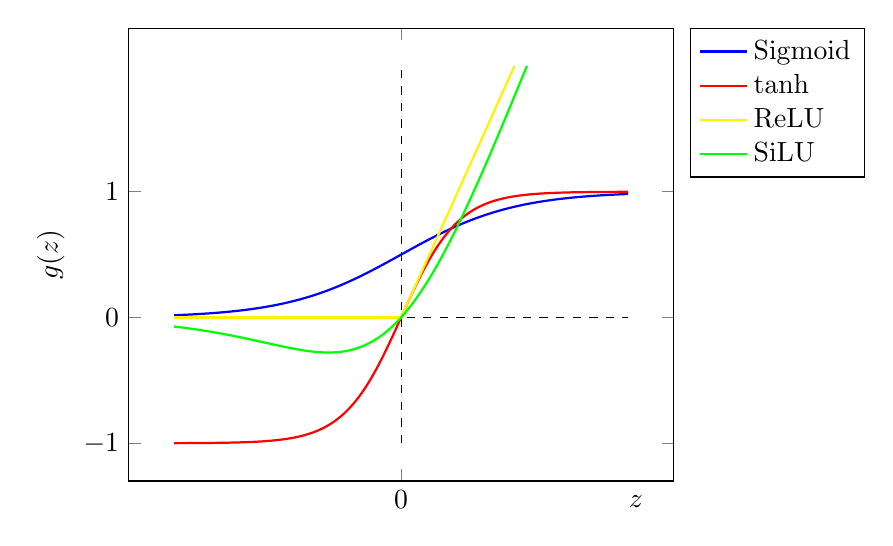
\begin{tikzpicture}
\pgfplotsset{width=8.5cm}
  \begin{axis}[
    domain=-4:4,
    xlabel=$z$,
    ylabel=$g(z)$,
    xtick={0},
    ytick={-1,0,1},
    every axis x label/.style={at={(0.9,-0.01)},anchor=north west},
    legend pos=outer north east,
    legend cell align=left
  ]
  % origin lines
  \addplot +[mark=none, black, dashed, forget plot] coordinates {(-4, 0) (4, 0)};
  \addplot +[mark=none, black, dashed, forget plot] coordinates {(0, -1) (0, 2)};

  % sigmoid 
  \addplot[thick, blue, samples=300] {1/(1+e^(-x))};%
  \addlegendentry{$\textnormal{Sigmoid}$}%

  % tanh
  \addplot[thick, red, samples=300] {tanh(x)};%
  \addlegendentry{$\textnormal{tanh}$}%
  
  % ELU
  %\addplot[thick, blue, samples=300, domain=-4:0, forget plot] {e^x - 1};%
  %\addplot[thick, blue, samples=300, domain=0:2] {x};%
  %\addlegendentry{$\textnormal{ELU}$}%

  % ReLU
  \addplot[thick, yellow, samples=300, domain=-4:0, forget plot] {0};%
  \addplot[thick, yellow, samples=300, domain=0:2] {x};%
  \addlegendentry{$\textnormal{ReLU}$}%

  % swish 
  % 1.278
  % 2.218
  \addplot[thick, green, samples=300, domain=-4:2.218] {x/(1+e^(-x))};%
  \addlegendentry{$\textnormal{SiLU}$}%

  \end{axis}%
\end{tikzpicture}
  \caption{
    The output of several common choices for the activation function $g(z)$ of an artificial neuron.
    The input $z$ is the output of the dot product between the activation and the weights, plus a bias term.
  }
  \label{fig:activation_functions}
\end{figure}


\subsubsection{Networks}

Several neurons are linked together in layers to form a neural network.
The inputs are propagated layer-by-layer through the network until reaching the final output layer.
The number of layers and neurons per layer are important hyperparameters (those parameters which are not optimised as part of the training process) which influence the performance of the model.
In the case of binary classification, the final output layer generally consists of a single neuron with a sigmoid activation 
%
\begin{equation}\label{eq:sigmoid}
  g(z) = \frac{1}{1 + e^{-z}} ,
\end{equation}
%
where $z$ is the output from the dot product of the inputs and the weights, plus the bias term.
The value $g(z)$ is bounded between zero and one allowing the final output to be interpreted as the probability that the input sample belongs to the signal class.
NNs have the crucial property of being differentiable functions, which facilitates the training process described in the next section.

%The activation $a_i^{(l)}$ is the output of the activation function $g(z)$ of the $i^{\text{th}}$ node in layer $l$. The tensor element $\Theta_{ji}^{(l)}$ is the weight connecting the $i^{\text{th}}$ node in layer $l - 1$ to the $j^{\text{th}}$ node in layer $l$. We can compute the outputs for each neuron in a layer simultaneously using ${a}_j^{(l)} = g(\Theta_{ji}^{(l)} a_i^{(l-1)})$, where the activation function is computed element wise on the vector. Computers can perform matrix operations in parallel, making a vectorised implementation such as this more efficient than calculating each output sequentially.

%Taking an item from the dataset $S$, $(\mathbf{x}_i, {y}_i)$, the input $\mathbf{x}_i$ is propagated through the network from left to right, one layer at a time. Finally, the classification result of the network, given by the output of the final neuron $\hat{\mathrm{y}} = h(\mathbf{x}_i)$, is obtained and can be compared to the true category of the data $\mathrm{y}_i$. 



\subsection{Training with Gradient Descent}\label{sec:training_sgd}

A training algorithm is used to optimise the weights and biases of a NN with exposure to the training data.
%The performance of the trained model depends on the amount and quality of the training data, and the efficacy of the training algorithm.
The training algorithm works by minimising a loss function $L$, which quantifies the error in the model's predictions.
NNs are commonly trained using backpropagation in combination with a variant of the stochastic gradient descent algorithm to iteratively update the model parameters.
In binary classification problems, the binary cross entropy loss
%
\begin{equation}\label{eq:bce_loss}
  L(x_i, \theta) = y_i \ln[f_\theta(x_i)] + (1 - y_i) \ln[1 - f_\theta(x_i)],
\end{equation}
%
is often used. Since the model $f$ is differentiable, a correction for each parameter $\theta_i$ can be computed by taking the partial derivative of $L$ with respect to the parameter.
Updated parameters $\theta_i'$ are calculated by updating the original parameter in the direction which reduces the loss.
%
\begin{equation}\label{eq:weight_update}
  \theta_i' = \theta_i - \alpha \pd{L}{\theta_i}
\end{equation}
%
The hyperparameter $\alpha$ is known as the \textit{learning rate} and dictates the size of the step taken in the direction of the slope. 
The errors for each parameter are efficiently calculated using the backpropagation algorithm \cite{rumelhart1986learning}.
The process of updating weights is repeated until the weights are judged to have converged, which means the network is trained.
In practice, small batches of the input data are shown to the network at a time. For each batch the average loss is calculated and the network's weights are updated.
There are many extensions and variations of the gradient descent algorithm.
This work uses the Adam optimiser which adds momentum to the weight updates (dampening oscillations) and an adaptive per-parameter learning rate \cite{2014arXiv1412.6980K}.

\begin{comment}
The gradient descent (\cref{sec:backprop_sgd}) algorithm is used to fit the model to the data.
Using \cref{eq:bce_loss}, an error for 
From \cref{eq:bce_loss}, the error on the output node can be 
The error for the final output node is computed first.
Errors for nodes in the previous layers are computed by \textit{backpropagating} this error through the network.
The error in the output node can be computed explicitly using the loss function in \cref{eq:bce_loss}.
To find the errors for the nodes in the preceding layers $\delta^{(L-1)}_i$, we need to differentiate eq. \ref{neural cost} with respect to $z^{(L-1)}_i$.
In order to perform the differentiation, we relate $z_1^{(L)} = g(z_j^{(L-1)}) \Theta_{1j}^{(L)}$.
The result,is tantamount to propagating the output error back through the network using the weights, and multiplying at each node by the derivative of the activation function. Once the errors have been propagated through the network, the partial derivatives of $J$ can be found using the final expression in eq. \ref{backprop defs}. Lastly the weights are updated simultaneously using eq. \ref{update weights}. 

gradient descent is an example of an \textit{optimisation} algorithm that minimises the cost function $J(\theta)$ (thereby fitting the logistic regression model discussed above to some data) by selecting the optimal values of $\theta$. The algorithm works by computing the partial derivatives of $J(\theta)$ with respect to the parameters $\theta$. The parameters are then altered slightly in the direction of decreasing slope, thereby reducing the cost function.
%The partial derivative of the loss function can be calculated for every parameter $\theta_i$ in the model.

The above step must be performed simultaneously for each $\theta_j$ in $\theta$, after which a new value of $J(\theta)$ can be calculated, and the process repeated. We can compute the partial derivatives of $J$ using the derivative of the logistic function from eq. \ref{eq:bce_loss}. The results are substituted into \cref{eq:weight_update} to obtain
\end{comment}



\section{Track Truth Origin Labelling}\label{sec:track_labelling}

Crucial to supervised learning techniques are the ground truth class labels which the machine learning model is trained to predict.
A set of track truth labels with a sufficient degree of granularity have been implemented in the \ATLAS software stack, and are listed in \cref{tab:truth_origins}.
The labelling scheme has been designed to be useful beyond the classification of good and fake tracks.
The origins are determined by analysing the simulated record to determine the physical process that led to the creation of the truth (i.e. simulated) particle which is  associated with each reconstructed track.
Tracks are associated with truth particles by selecting the particle with the highest \textit{truth-matching probability} (TMP), defined in \cref{eq:tmp_def}.
For a given truth particle, the TMP is a weighted sum of the number of hits on a reconstructed track which are matched to the truth particle $N^{\textnormal{match}}$, divided the total number of hits on the track $N^{\textnormal{total}}$.
The weights are sub-detector-dependent and are designed to account for the varying importance of the different ID sub-detectors (based upon their precision) in the reconstruction of a track.
%
\begin{equation}\label{eq:tmp_def}
    \textnormal{TMP} = 
    \frac{
        10 N_{\textnormal{Pix}}^{\textnormal{match}} + 
        5  N_{\textnormal{SCT}}^{\textnormal{match}} + 
           N_{\textnormal{TRT}}^{\textnormal{match}}
        }{
        10 N_{\textnormal{Pix}}^{\textnormal{total}} + 
        5  N_{\textnormal{SCT}}^{\textnormal{total}} + 
            N_{\textnormal{TRT}}^{\textnormal{total}}
        }
\end{equation}
%
For the fake track classification tool, the track truth origins in \cref{tab:truth_origins} are used to construct a binary label by assigning all fake tracks to the background category, and all other tracks as signal.
The fake track classifier is then trained to distinguish between these two categories of tracks.
Fake tracks are defined using the TMP, with a $\textnormal{TMP} < 0.75$\footnote{An alternative definition of a fake track as one with $\textnormal{TMP} < 0.5$ is also in use within ATLAS, but 0.75 was used for this study.}
giving a track the label of fake.
Fake tracks are made up of combinatorial fakes, which are tracks which do not correspond to the trajectory of any truth particle, and poorly reconstructed tracks, which may somewhat resemble the trajectory of a truth particle but due to the presence of some wrong hits on the track will not accurately reproduce the true trajectory.
In such cases the fake track can still be identified as having an origin: it is for example possible to have a fake track which is from the decay of a \bhadron.


\begin{table}[!htbp]
    \footnotesize\centering
    \setlength{\tabcolsep}{0.5em} % for the horizontal padding
    \begin{tabular}{lll}
        \toprule\hline
        \textbf{Truth Origin} & \textbf{Description} \\
        \hline
        Pile-up  & From a \pp collision other than the primary interaction \\
        Fake    & Created from the hits of multiple particles \\
        Primary & Does not originate from any secondary decay \\
        fromB   & From the decay of a \bhadron \\
        fromBC  & From a \chadron decay which itself is from the decay of a \bhadron \\
        fromC   & From the decay of a \chadron which is not from the decay of a \bhadron \\
        %fromTau & From the decay of a $\tau$ \\
        OtherSecondary & From other secondary interactions and decays \\
        \hline\bottomrule
    \end{tabular}
    \caption{
      Truth origins which are used to categorise the physical process that led to the production of a track.
      Tracks are matched to charged particles using the truth-matching probability~\cite{PERF-2015-08}.
      A truth-matching probability of less than $0.75$ indicates that reconstructed track parameters are likely to be mismeasured and may not correspond to the trajectory of a single charged particle.
      The ``OtherSecondary'' origin includes tracks from photon conversions, \Kshort and $\Lambda^0$ decays, and hadronic interactions.
    }
    \label{tab:truth_origins}
\end{table}

\section{Fake Track Identification Tool}\label{sec:fake_track_mva}

The rate of fake tracks increases at high transverse momentum as shown in \cref{fig:fakerate_vs} due to the difficulties in track reconstruction outlined in \cref{sec:b_had_reco_chall}.
The performance of \btagging algorithms is reduced as a direct result of the presence of these tracks as shown for SV1 (see \cref{sec:vertex_reco}) in \cref{fig:sv1_perf_nofake}, where the efficiency to mistag a \ljet decreases by up to \pct{35} at a \beff of \pct{35} if such tracks are removed.


\begin{figure}[!htbp]
  \centering
  \begin{subfigure}[b]{0.48\textwidth}
      \centering
      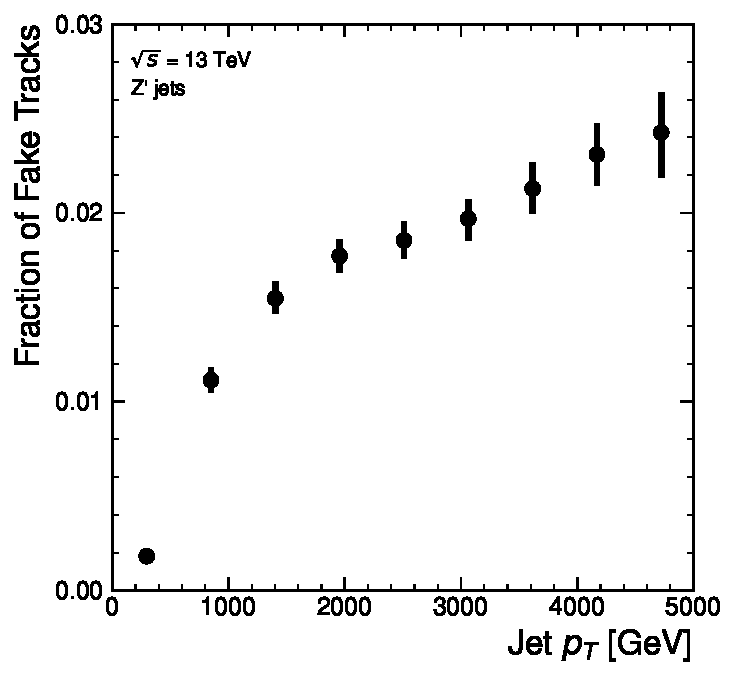
\includegraphics[width=\textwidth]{chapters/4.track_classifier/figs/fake_vs_pt.pdf}
  \end{subfigure}
  \quad
  \begin{subfigure}[b]{0.48\textwidth}
      \centering
      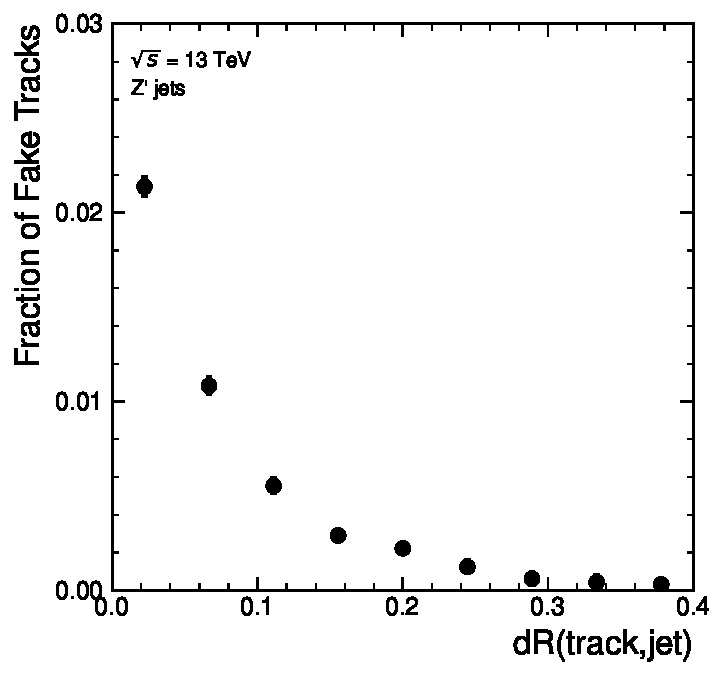
\includegraphics[width=\textwidth]{chapters/4.track_classifier/figs/fake_vs_dr.pdf}
  \end{subfigure}
  \caption{
    Rate of fake tracks as a function of jet transverse momentum (left) and $\DeltaR(\textnormal{track}, \textnormal{jet})$ (right) for jets in the \Zprime sample.
    The rate of fake tracks increases significantly as a function of \pt, and also increases as the distance to the jet axis decreases.
  }
  \label{fig:fakerate_vs}
\end{figure}

\begin{figure}[!htbp]
    \centering
    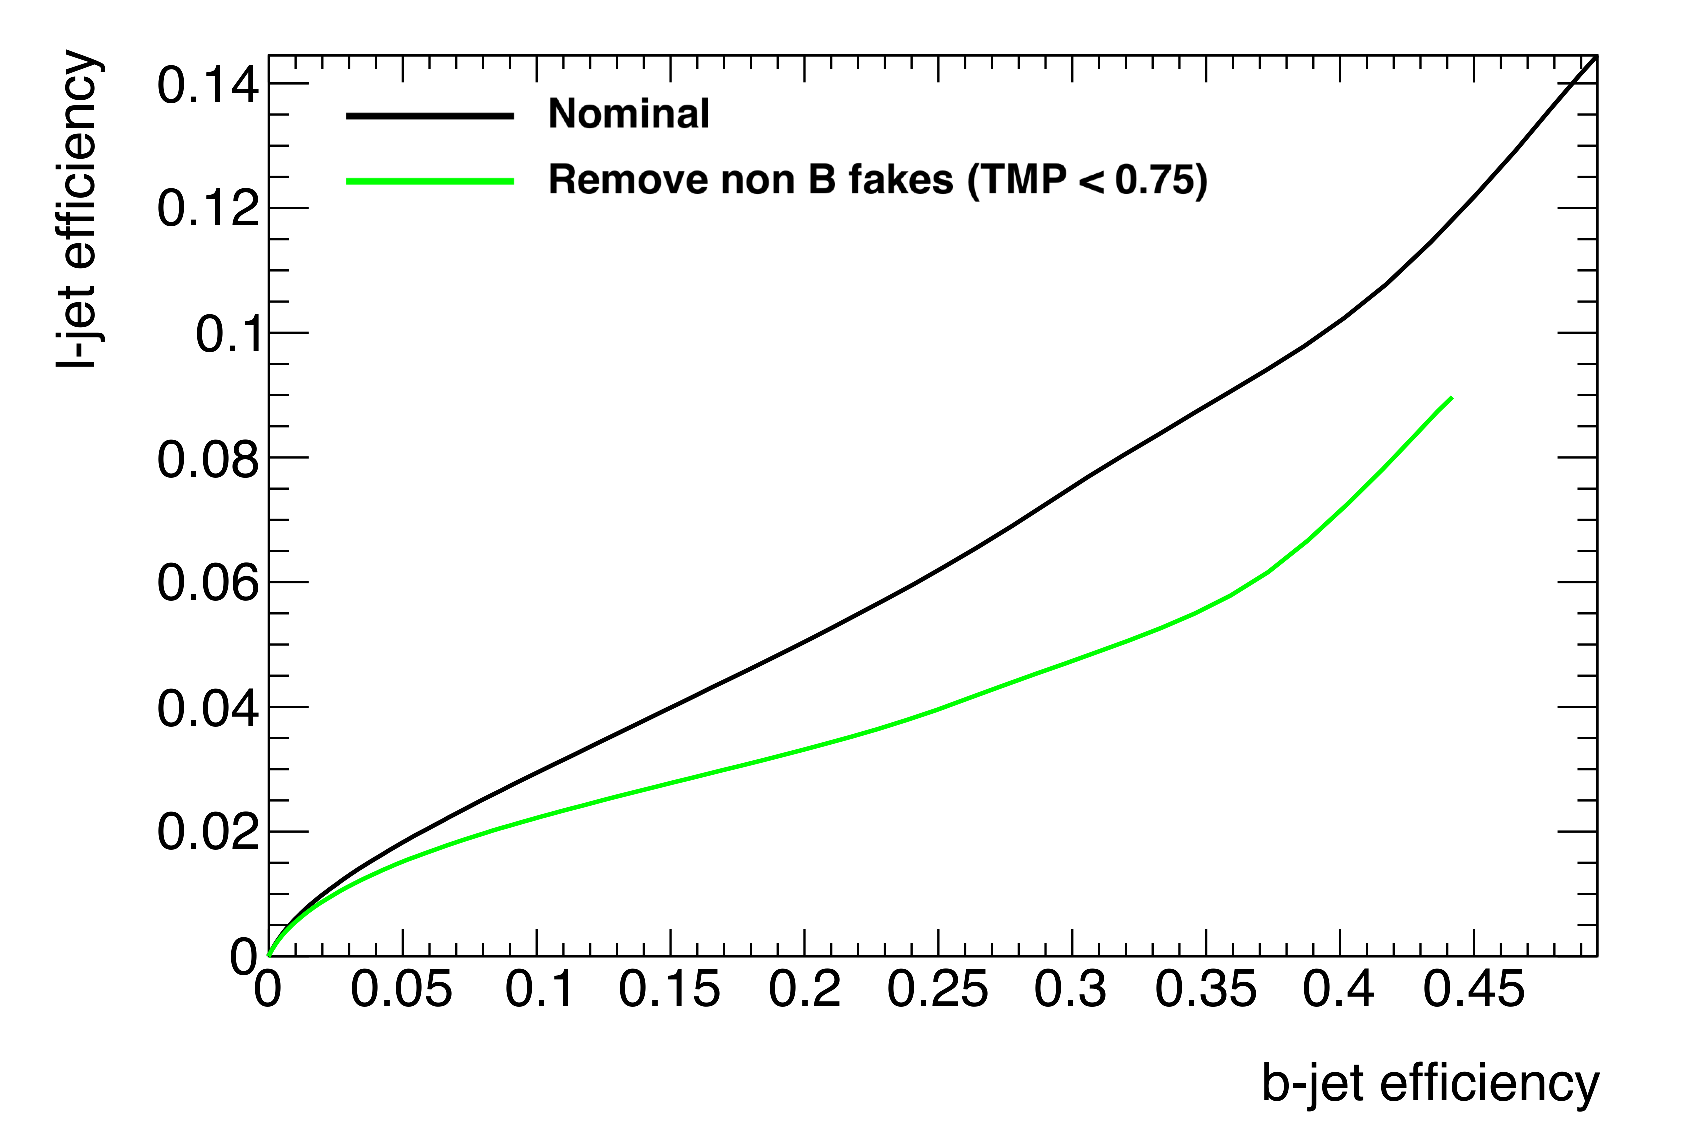
\includegraphics[width=0.7\textwidth]{chapters/4.track_classifier/figs/sv1_perf_nofake.pdf}
    \caption{
      The \ljet efficiency of the low level tagger SV1 for \Zprimejets with \Zprimept, as a function of \bjet efficiency.
      The nominal tracking setup (black) is shown alongside the case where fake tracks which are not from the decay of a \bhadron are removed.
      The \ljet efficiency is decreased, demonstrating that the presence of fake tracks is detrimental to the algorithm performance.
    }
    \label{fig:sv1_perf_nofake}
\end{figure}

To identify and remove fake tracks, a NN classification tool was trained with all non-fake tracks as the signal class and fake tracks as the background class.
Inputs to the model are described in \cref{sec:fake_mva_model_inputs}, while fake track removal performance is given in \cref{sec:fake_track_mva_results}.
Both models are trained and evaluated using tracks associated to jets from the \ttbar and \Zprime samples described in \cref{sec:track_classifier_datasets}.
\ttbarjets made up \pct{70} of the jets used for training, with the remaining \pct{30} coming from \Zprimejets.


\subsection{Model Inputs}\label{sec:fake_mva_model_inputs}

%\newcommand{\ipdefsfootnote}{%
%Impact parameter significances are defined as the IP divided by its corresponding uncertainty, $\dzerosig = d_0 / \dzerouncert$ and $\zzerosig = z_0 / \zzerouncert$.
%Track IP significances are lifetime signed according to the track's direction with respect to the jet axis and the primary vertex \cite{PERF-2012-04}.
%}

The fake track NN is given two jet variables and 20 tracking related variables for each track fed into the network.
The jet transverse momentum and signed pseudorapidity constitute the jet-level inputs, with the track-level inputs listed in \cref{tab:fake_mva_track_inputs}.


\begin{table}[!htbp]
  \footnotesize\centering
  \setlength{\tabcolsep}{0.5em} % for the horizontal padding
  \begin{tabular}{ll}
    \toprule\hline
    \textbf{Jet Input} & \textbf{Description} \\
    \hline
    $\pt$ & Jet transverse momentum \\
    $\eta$ & Signed jet pseudorapidity \\
    \toprule
    \textbf{Track Input} & \textbf{Description} \\
    \hline
    $\pt$ & Track transverse momentum \\
    $\DeltaR$ & Angular distance between the track and jet \\
    $d_0$  & Closest distance from the track to the PV in the longitudinal plane \\
    $z_0$  & Closest distance from the track to the PV in the transverse plane \\
    nIBLHits   & Number of IBL hits \\
    nPixHits   & Number of pixel hits \\
    nSCTHits   & Number of SCT hits \\
    nTRTHits   & Number of TRT hits \\
    nBLHits    & Number of B-layer hits \\
    nIBLShared & Number of shared IBL hits \\
    nIBLSplit  & Number of split IBL hits \\
    nPixShared & Number of shared pixel hits \\
    nPixSplit  & Number of split pixel hits \\
    nSCTShared & Number of shared SCT hits \\
    $r_{\textnormal{first}}$      & Radius of first hit \\
    nDOF   & Number of degrees of freedom on the track \\
    FracRank & Ambiguity solver ordering variable \\
    \hline\bottomrule
  \end{tabular}
  \caption{
    Input features to the fake track classification NN.
    Basic jet kinematics, along with information about the reconstructed track parameters and constituent hits are used.
    Shared hits, are hits used on multiple tracks which have not been classified as split by the cluster-splitting neural networks~\cite{PERF-2015-08}, while split hits are hits used by multiple tracks which have been identified as merged, and therefore split.
    ``Primary vertex'' (defined in \cref{sec:vertex_reco}) is abbreviated as PV.
  }
  \label{tab:fake_mva_track_inputs}
\end{table}

The track parameters and hit pattern are key indicators of whether or not a track is fake.
The FracRank variable is the ordered index of the tracks that pass the ambiguity solver's selection divided by the total number of successfully reconstructed tracks in the event.
The ambiguity solver processes track candidates iteratively in order of an internal score (see \cref{sec:track_reco}), and the order in which tracks are accepted is preserved.
Since tracks with shared hits have lower scores, tracks which do not require the removal of shared hits are likely to be processed and accepted earlier on, whereas tracks with shared hits will be processed later and potentially have their shared hits removed.
Hence the FracRank variable gives an indication of the track quality and how likely it is that hits would have been removed (tracks processed later on are more likely to have hits removed).

Track selection follows the loose selection described in \rcite{ATL-PHYS-PUB-2020-014} and outlined in \cref{tab:fake_track_mva_selections}, which was found to improve the performance compared to previous tighter selections, whilst ensuring good resolution of the track's parameters and a low fake rate \cite{PERF-2015-08}.
Inputs are scaled to have a central value of zero and a variance of unity before training and evaluation.


\subsection{Model Hyperparameters}\label{sec:hyperparameters}

Due to the imbalance between the two classes (with fake tracks being relatively uncommon), a weight was added to the loss function for the background class to balance their relative weights.
The NN was made up of two hidden layers with 220 nodes per layer.
The ReLU activation function was used in conjunction with the Adam optimiser with a learning rate of $1\text{e}{-3}$.
Optimisation of the networks architecture was carried out to ensure optimal performance with a relatively small number of learnable parameters -- 54,000.
The model was trained using \num{40} million tracks with a further \num{4} million tracks each used for validation and testing.
The number of tracks used for training was found to be sufficient to maximise the performance of the model, with no improvement observed when using more tracks.
A full list of the model hyperparameters is given in \cref{tab:fake_track_mva_hyperparams}.

\begin{table}[!htbp]
  \footnotesize\centering
  \setlength{\tabcolsep}{0.5em} % for the horizontal padding
  \begin{tabular}{lll}
      \toprule\hline
      \textbf{Hyperparameter} & \textbf{Value} \\
      \hline
      Batch size & 2048 \\
      Activation & ReLU \\
      Optimiser & Adam \\
      Initial learning rate & $1\text{e}{-3}$ \\
      Training epochs & 20 \\
      Training tracks & 40m \\
      Validation tracks & 4m \\
      Testing tracks & 4m \\
      \hline\bottomrule
  \end{tabular}
  \caption{
    Hyperparameters for the track classification model.
  }
  \label{tab:fake_track_mva_hyperparams}
\end{table}


\subsection{Results}\label{sec:fake_track_mva_results}


In order to evaluate the fake track classification tool, a orthogonal test sample of $4$ million tracks in jets in the combined \ttbar and \Zprime samples was used.
The continuous scalar output from the NN model is interpreted as the probability that a given track is a signal track (i.e. not fake).
\cref{fig:track_classifier_output_roc} shows the performance of the fake track classification NN. The signal and background classes are well separated in the output of the tool.
Also shown is a receiver operating characteristic (ROC) curve, which plots the rate of true positives against the rate of false positives over a scan of cut points on the NN output ranging from zero to one.
The area under the curve (AUC) gives a summary of the aggregate classification power of the model.
The fake track classification tool achieves an AUC of $0.935$ for all tracks, which is indicative of a well-performing model.
Considering only tracks from \bhadron decays, this value drops slightly to $0.928$. 

\begin{figure}[!htbp]
  \centering
  \begin{subfigure}[b]{0.48\textwidth}
      \centering
      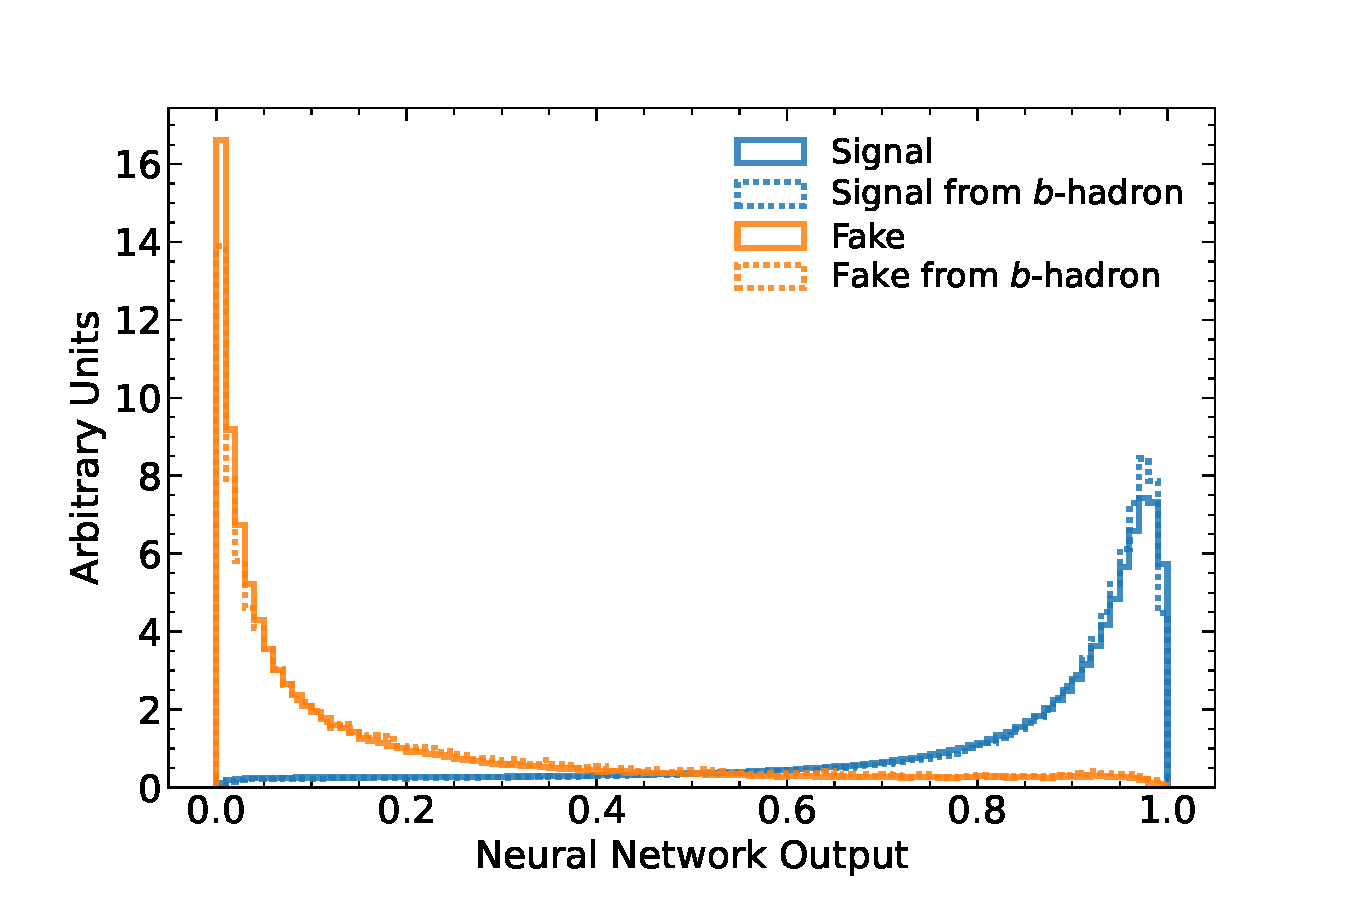
\includegraphics[width=\textwidth]{chapters/4.track_classifier/figs/fake_id_output.pdf}
  \end{subfigure}
  \quad
  \begin{subfigure}[b]{0.48\textwidth}
      \centering
      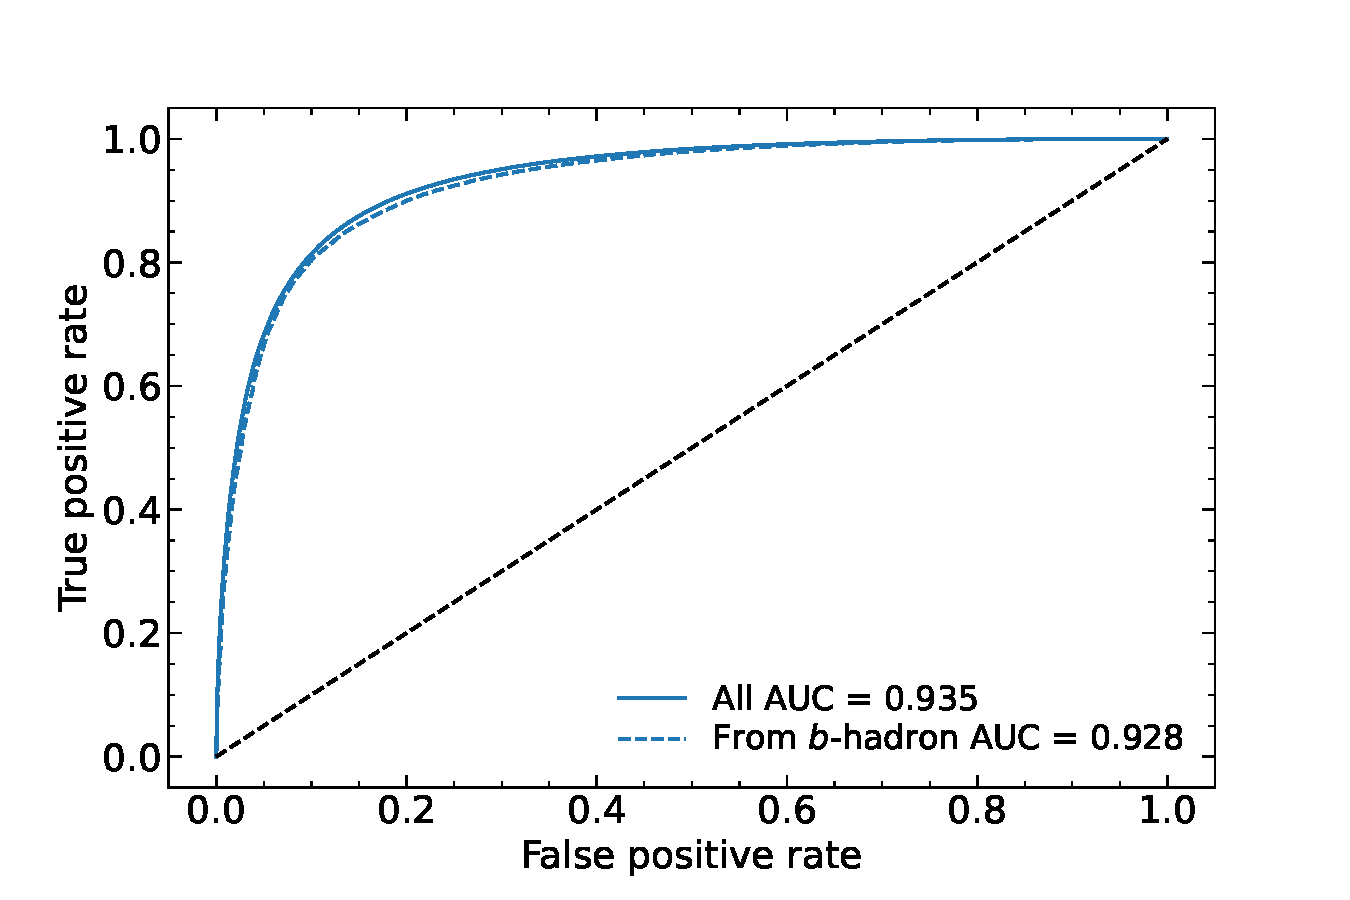
\includegraphics[width=\textwidth]{chapters/4.track_classifier/figs/fake_id_roc.pdf}
  \end{subfigure}
  \caption{
    (left) Normalised histograms of the fake track classification model output separated for signal and fake tracks, and further separated by those tracks which are from the decay of a \bhadron.
    (right) The ROC curve for all tracks (solid line) and tracks from the decay of a \bhadron (dashed line).
    The plots show tracks in the combined \ttbar and \Zprime testing sample.
    The model is able to successfully discriminate between signal and fake tracks, and shows a very similar performance when looking specifically at tracks from the decay of a \bhadron.
  }
  \label{fig:track_classifier_output_roc}
\end{figure}

Signal and fake track efficiencies at two different NN output cut points are shown in \cref{tab:fake_track_mva_effs}.
The results demonstrate that the tool is effective in retaining \pct{98.8} of signal tracks, while correctly identifying (and therefore enabling the removal of) \pct{45.6} of fake tracks.
\cref{tab:fake_track_mva_effs} also shows that a significant amount of tracks which are labelled as both fake and from the decay of a \bhadron are also removed.
This can happen because fake tracks with $\textnormal{TMP} < 0.75$ are still matched to a truth particle, which can be the decay product of a \bhadron.

\begin{table}[!htbp]
  \footnotesize\centering
  \setlength{\tabcolsep}{0.5em} % for the horizontal padding
  \begin{tabular}{ccccc}
      \toprule\hline
      \multirow{2}{2cm}{NN Output Cut} & \multicolumn{2}{c}{\textbf{Signal Track Efficiency}} & \multicolumn{2}{c}{\textbf{Fake Track Recall}} \\
      & All & From $b$ & All & From $b$ \\
      \hline
      0.06 & \pct{98.8} & \pct{98.9} & \pct{45.6} & \pct{39.8} \\
      0.12 & \pct{97.3} & \pct{97.5} & \pct{59.4} & \pct{53.6} \\
      \hline\bottomrule
  \end{tabular}
  \caption{
    Good and fake track selection efficiencies for the combined \ttbar and \Zprime samples.
    Two working points are defined, cutting on the NN output at $0.06$ and $0.12$.
  }
  \label{tab:fake_track_mva_effs}
\end{table}

\section{\bhadron Track Identification}

After initial tests and investigation, it was found that fake tracks which were the result of \bhadron decays actually aided \btagging performance, as demonstrated in \cref{fig:track_mva_sv1}.
The application of a single tool which removed all fake tracks was therefore not optimal.
A second tool was therefore trained in the same manner as the first, this one was designed to distinguish between those tracks which were from the decay of a \bhadron (FromB and FromBC in \cref{tab:truth_origins}) and those which were not (all other truth origins).
Fake tracks which were from the decay of a \bhadron were included in the signal class.
The \bhadron decay track NN was trained using the same setup as described above, with the same tracks, input variables, and training procedure.
The performance of the model to separate \bhadron decay tracks from other tracks is shown in \cref{fig:b_id_output_roc}.
Using a selection WP of 0.1, the model can retain \pct{98.5} of \bhadron tracks and reject \pct{46.2} of tracks not from the decay of a \bhadron.
In \cref{sec:mva_combined}, this model is used in conjunction with the fake track identification NN to identify and remove fake tracks which are not from the decay of a \bhadron.

% TODO: ADD TABLE REQUEST 

\begin{figure}[!htbp]
  \centering
  \begin{subfigure}[b]{0.48\textwidth}
      \centering
      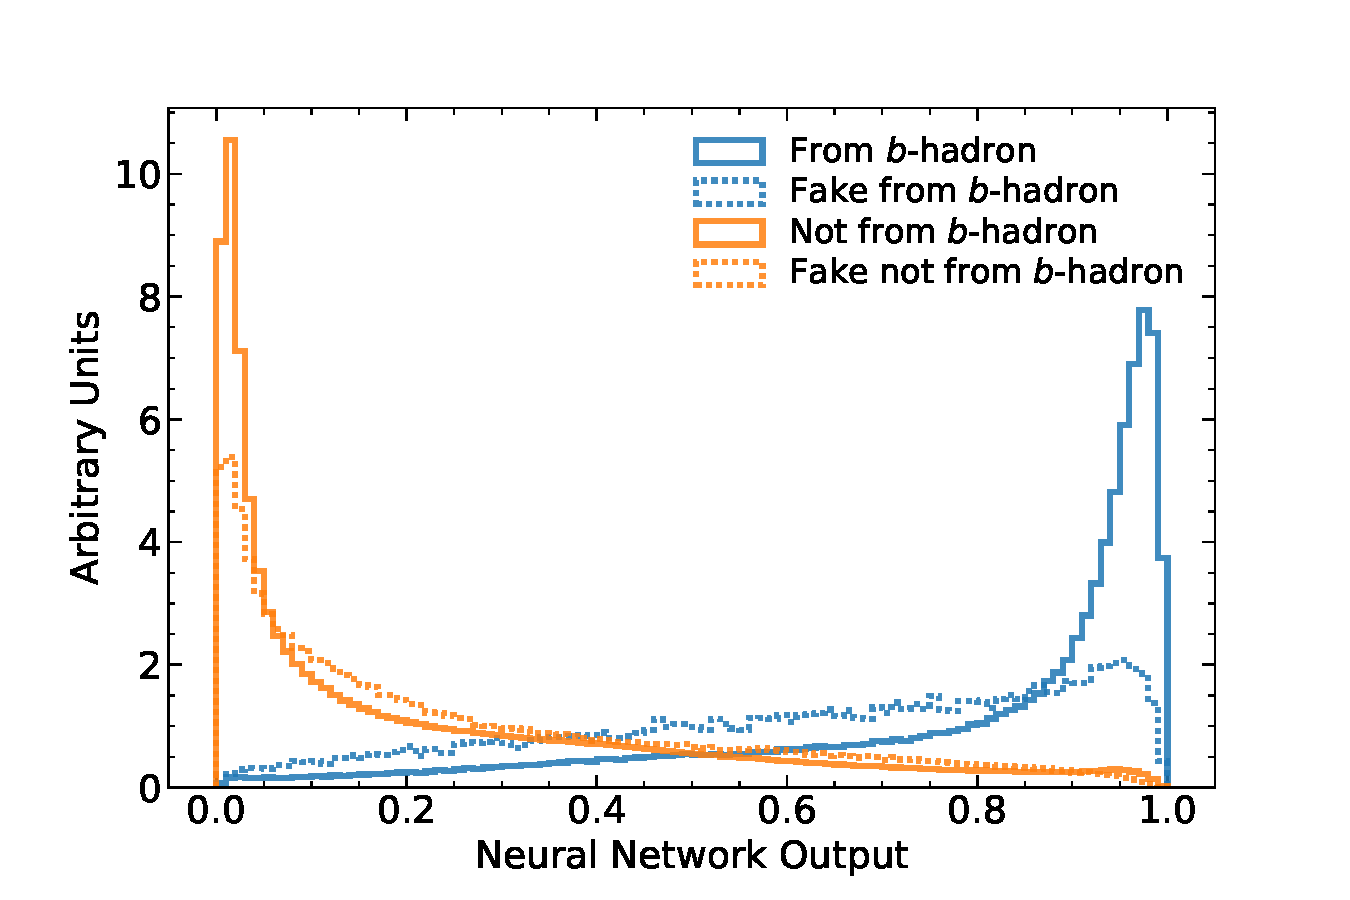
\includegraphics[width=\textwidth]{chapters/4.track_classifier/figs/b_id_output.pdf}
  \end{subfigure}
  \quad
  \begin{subfigure}[b]{0.48\textwidth}
      \centering
      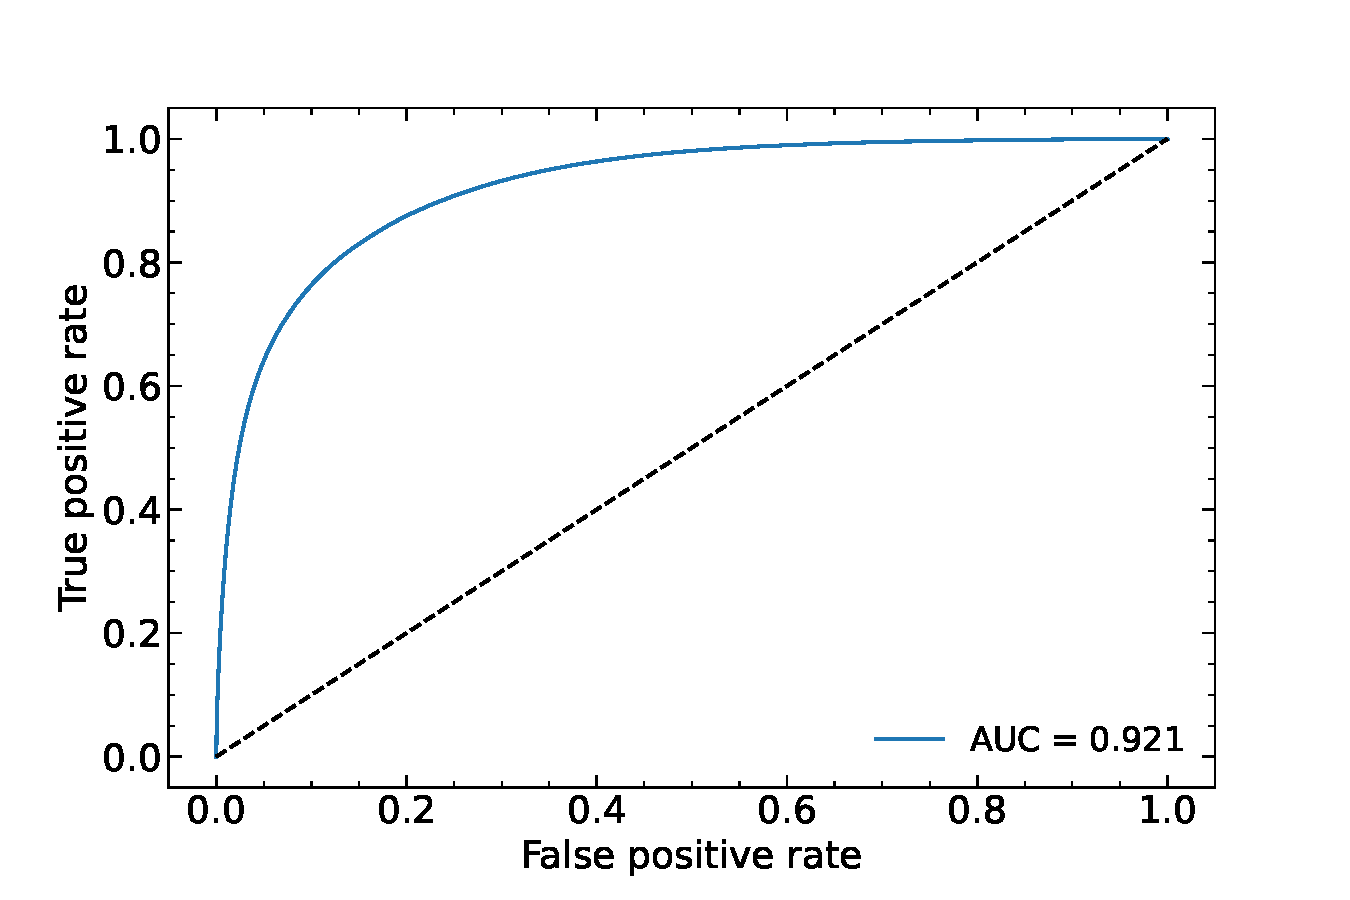
\includegraphics[width=\textwidth]{chapters/4.track_classifier/figs/b_id_roc.pdf}
  \end{subfigure}
  \caption{
    (left) Normalised histogram of the \bhadron track identification model output separated for tracks from the decay of a \bhadron and tracks from other sources.
    The two groups are further separated into those tracks which are fake.
    (right) The ROC curve for all tracks (solid line).
    The plots show tracks in the combined \ttbar and \Zprime testing sample.
  }
  \label{fig:b_id_output_roc}
\end{figure}


\section{Combined Approach}\label{sec:mva_combined}


A 2-dimensional cut was then used to only reject those tracks that had a high probability of being fake, and also a low probability of being a \bhadron decay track.
The results of the combined approach are provided in \cref{tab:combined_va}, which shows that for the working point ``A'', \pct{98.6} of \bhadron decay tracks (both good and fake) are retained, while \pct{50.7} of fake tracks which are not from \bhadron decays are rejected.

\begin{table}[!htbp]
  \footnotesize\centering
  \setlength{\tabcolsep}{0.5em} % for the horizontal padding
  \begin{tabular}{l>{\raggedright}p{2cm}>{\raggedright}p{2cm}>{\raggedright}p{4cm}>{\raggedright\arraybackslash}p{4cm}}
      \toprule\hline
      \textbf{WP} & \textbf{Fake NN Cut} & \textbf{\bhadron Decay NN Cut} & \textbf{Retained \bhadron Tracks} & \textbf{Fake non-\bhadron Tracks Rejected} \\
      \hline
      A & 0.5 & 0.4 & \pct{98.6} & \pct{50.7} \\
      B & 0.6 & 0.5 & \pct{97.5} & \pct{62.0} \\
      \hline\bottomrule
  \end{tabular}
  \caption{
    Cut values for the fake and \bhadron decay track NNs for the two defined working points.
    Working point ``B'' cuts more aggressively on the NN outputs than WP ``A'', removing more fake tracks but resulting in an increased loss of signal tracks (which here are all \bhadron decay tracks).
  }
  \label{tab:combined_va}
\end{table}
%// cut A: B tracks kept = 98.6% (99.4% of good B tracks and 84.8% of fake B tracks). Non B Fakes Rejected: 50.7%
%// cut B: B tracks kept = 97.5% (98.4% of good B tracks and 80.8% of fake B tracks). Non B Fakes Rejected: 62.0%

The \ljet efficiency of SV1 is successfully reduced when using the combined tools to remove fake tracks that are not from a \bhadron decay, as shown in \cref{fig:track_mva_sv1}.
At a \beff of \pct{70}, the \ljet mistag rate for jets with $250 < \pt < \SI{400}{\GeV}$ is reduced from $0.054$ to $0.044$, a relative improvement of approximately \pct{20}.
For jets with $400 < \pt < \SI{1000}{\GeV}$ the mistag rate drops from 0.1 to 0.08 for a similar relative improvement of \pct{20}.
The performance of the fake track removal approach was also tested for the other low level vertexing algorithm -- JetFitter.
A similar level of improvement in the \ljet mistag rate was observed with a reduction of up to a \pct{20} reduction for both low- and \highpt \Zprimejets achieved.
Together, these results demonstrate that by identifying and removing fake tracks which are not the result of the weak decay of a \bhadron, the performance of the low level tagging algorithms can be improved by an amount which is comparable to the improvement that would be observed if the tracks were selected at truth level1.

\begin{figure}[!htbp]
  \centering
  \begin{subfigure}[b]{0.48\textwidth}
      \centering
      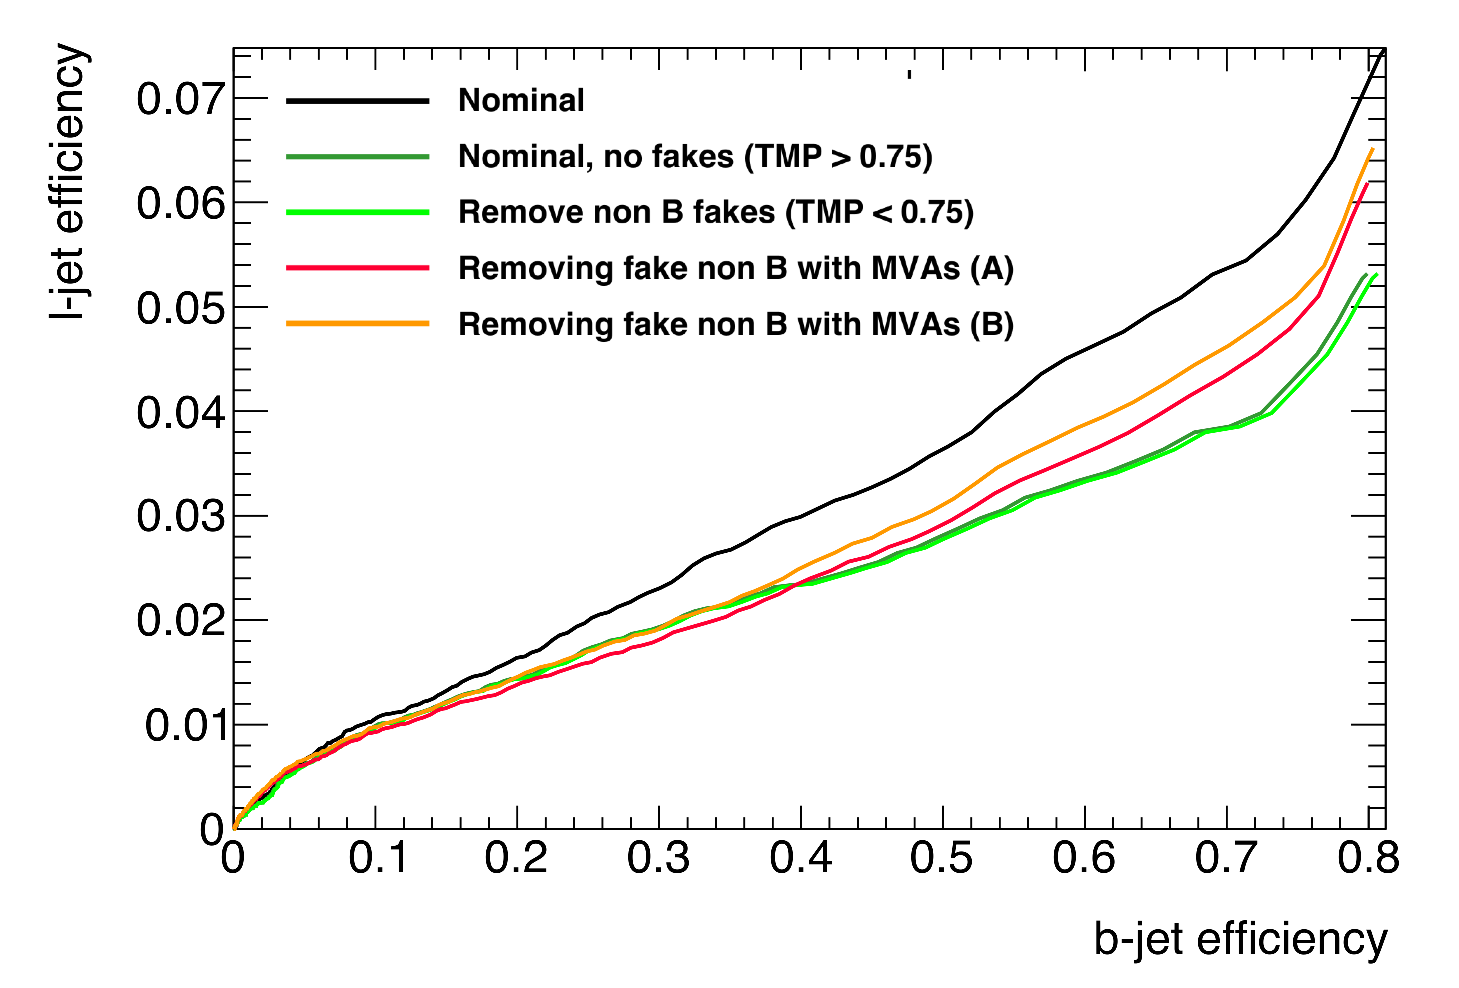
\includegraphics[width=\textwidth]{chapters/4.track_classifier/figs/sv1_mva_lowpt.pdf}
  \end{subfigure}
  \quad
  \begin{subfigure}[b]{0.48\textwidth}
      \centering
      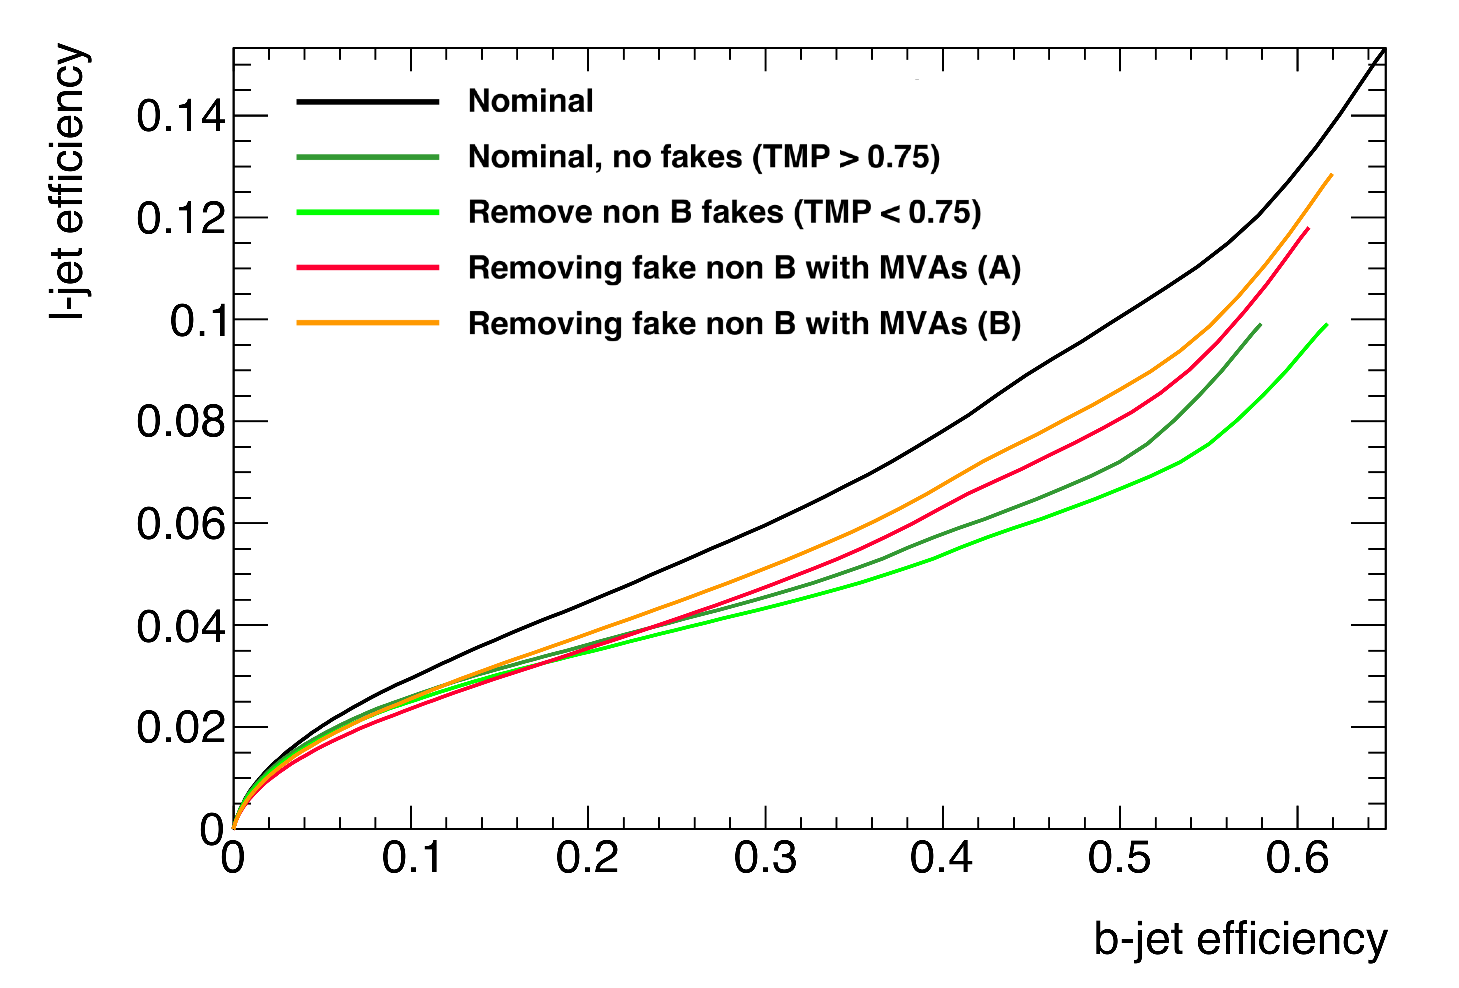
\includegraphics[width=\textwidth]{chapters/4.track_classifier/figs/sv1_mva_hipt.pdf}
  \end{subfigure}
  \caption{
    The effect of applying the fake track identification algorithm together with the \bhadron decay track identification on the jet tagging performance of SV1 for \Zprimejets with $\SI{250}{\GeV} < \pt < \SI{400}{\GeV}$ (left) and $\SI{400}{\GeV} < \pt < \SI{1}{\TeV}$ (right).
    The nominal SV1 \ljet efficiency (black) is compared to two working points of fake track removal, labelled ``A'' (red) and ``B'' (orange), which represent two different 2D working points of the track classification tools.
    Removal of fake tracks based on truth information is shown by the green curves.
  }
  \label{fig:track_mva_sv1}
\end{figure}

%\begin{figure}[!htbp]
%  \centering
%  \begin{subfigure}[b]{0.48\textwidth}
%      \centering
%      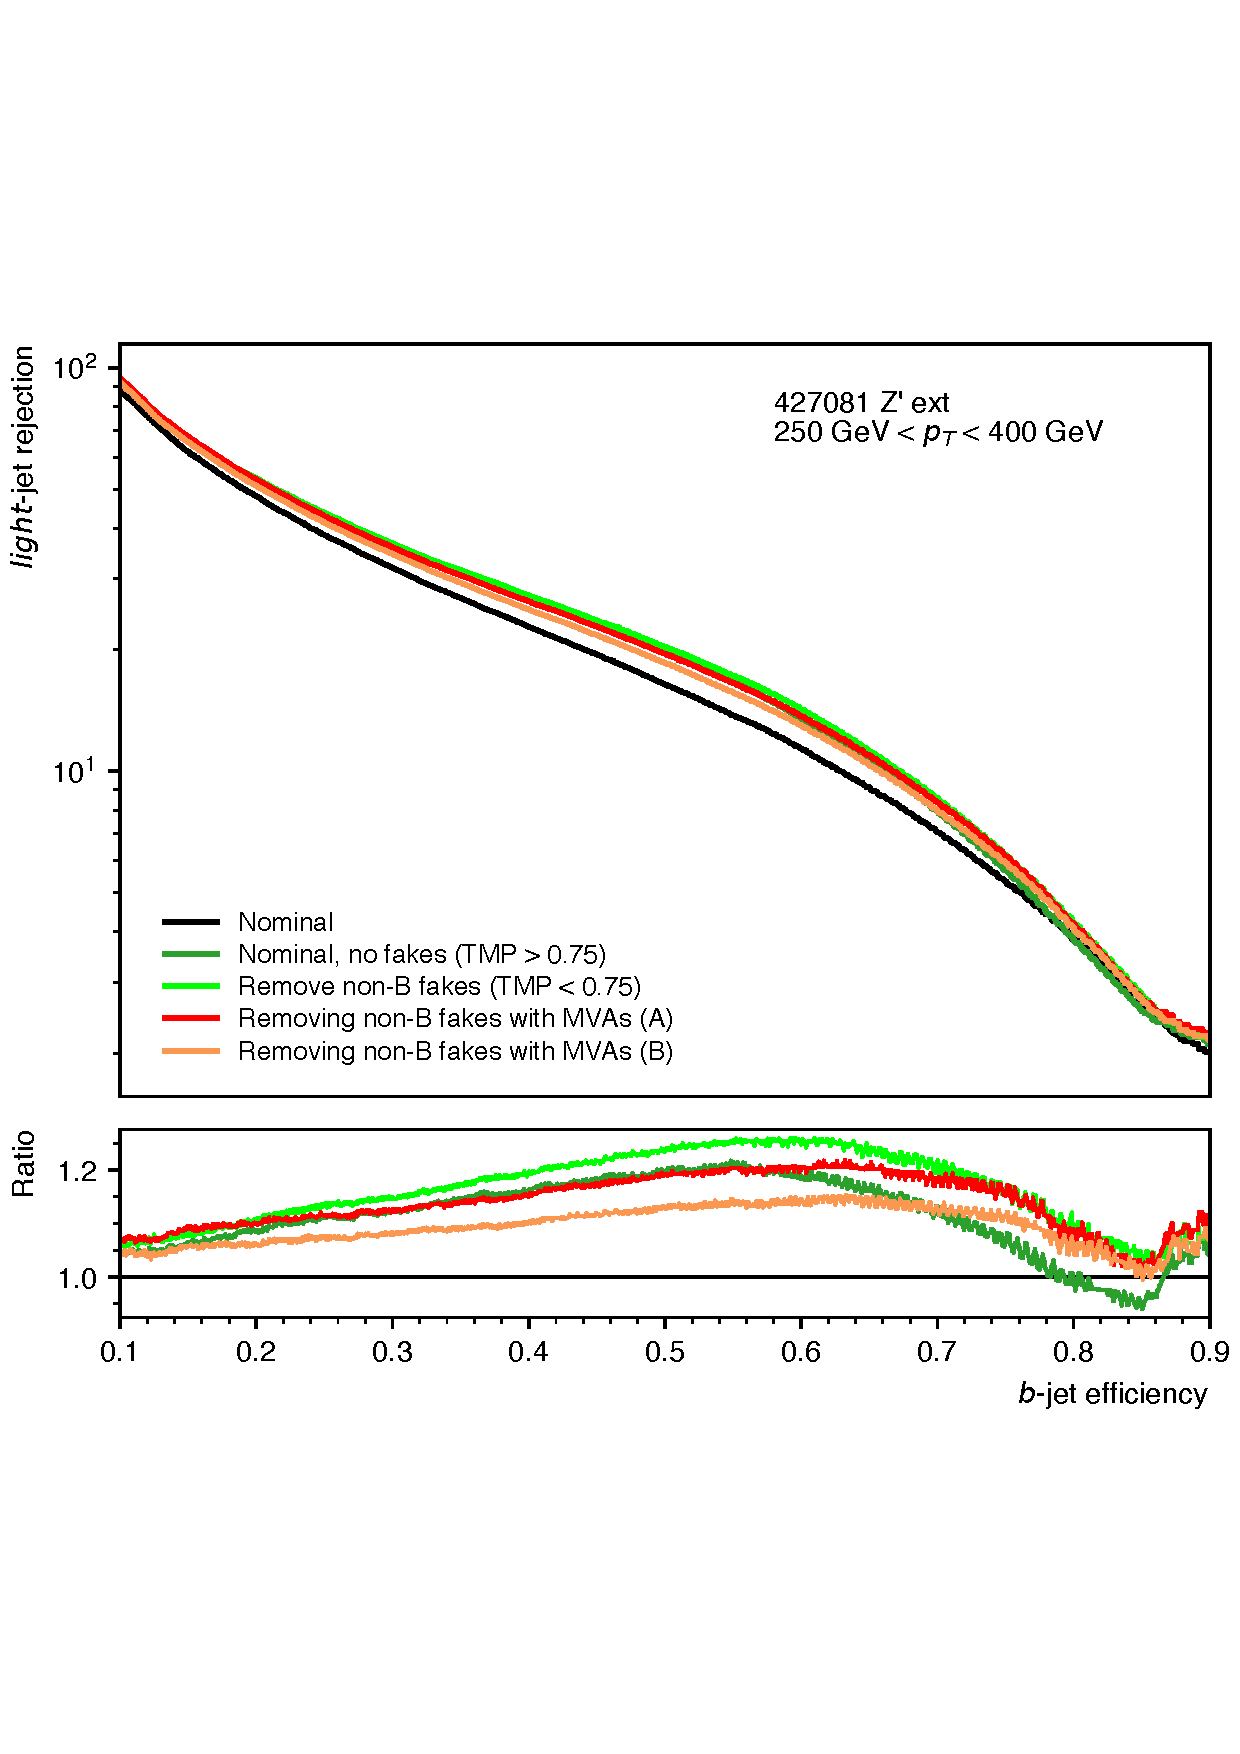
\includegraphics[width=\textwidth]{chapters/4.track_classifier/figs/zprime_jf_lowpt.pdf}
%  \end{subfigure}
%  \quad
%  \begin{subfigure}[b]{0.48\textwidth}
%      \centering
%      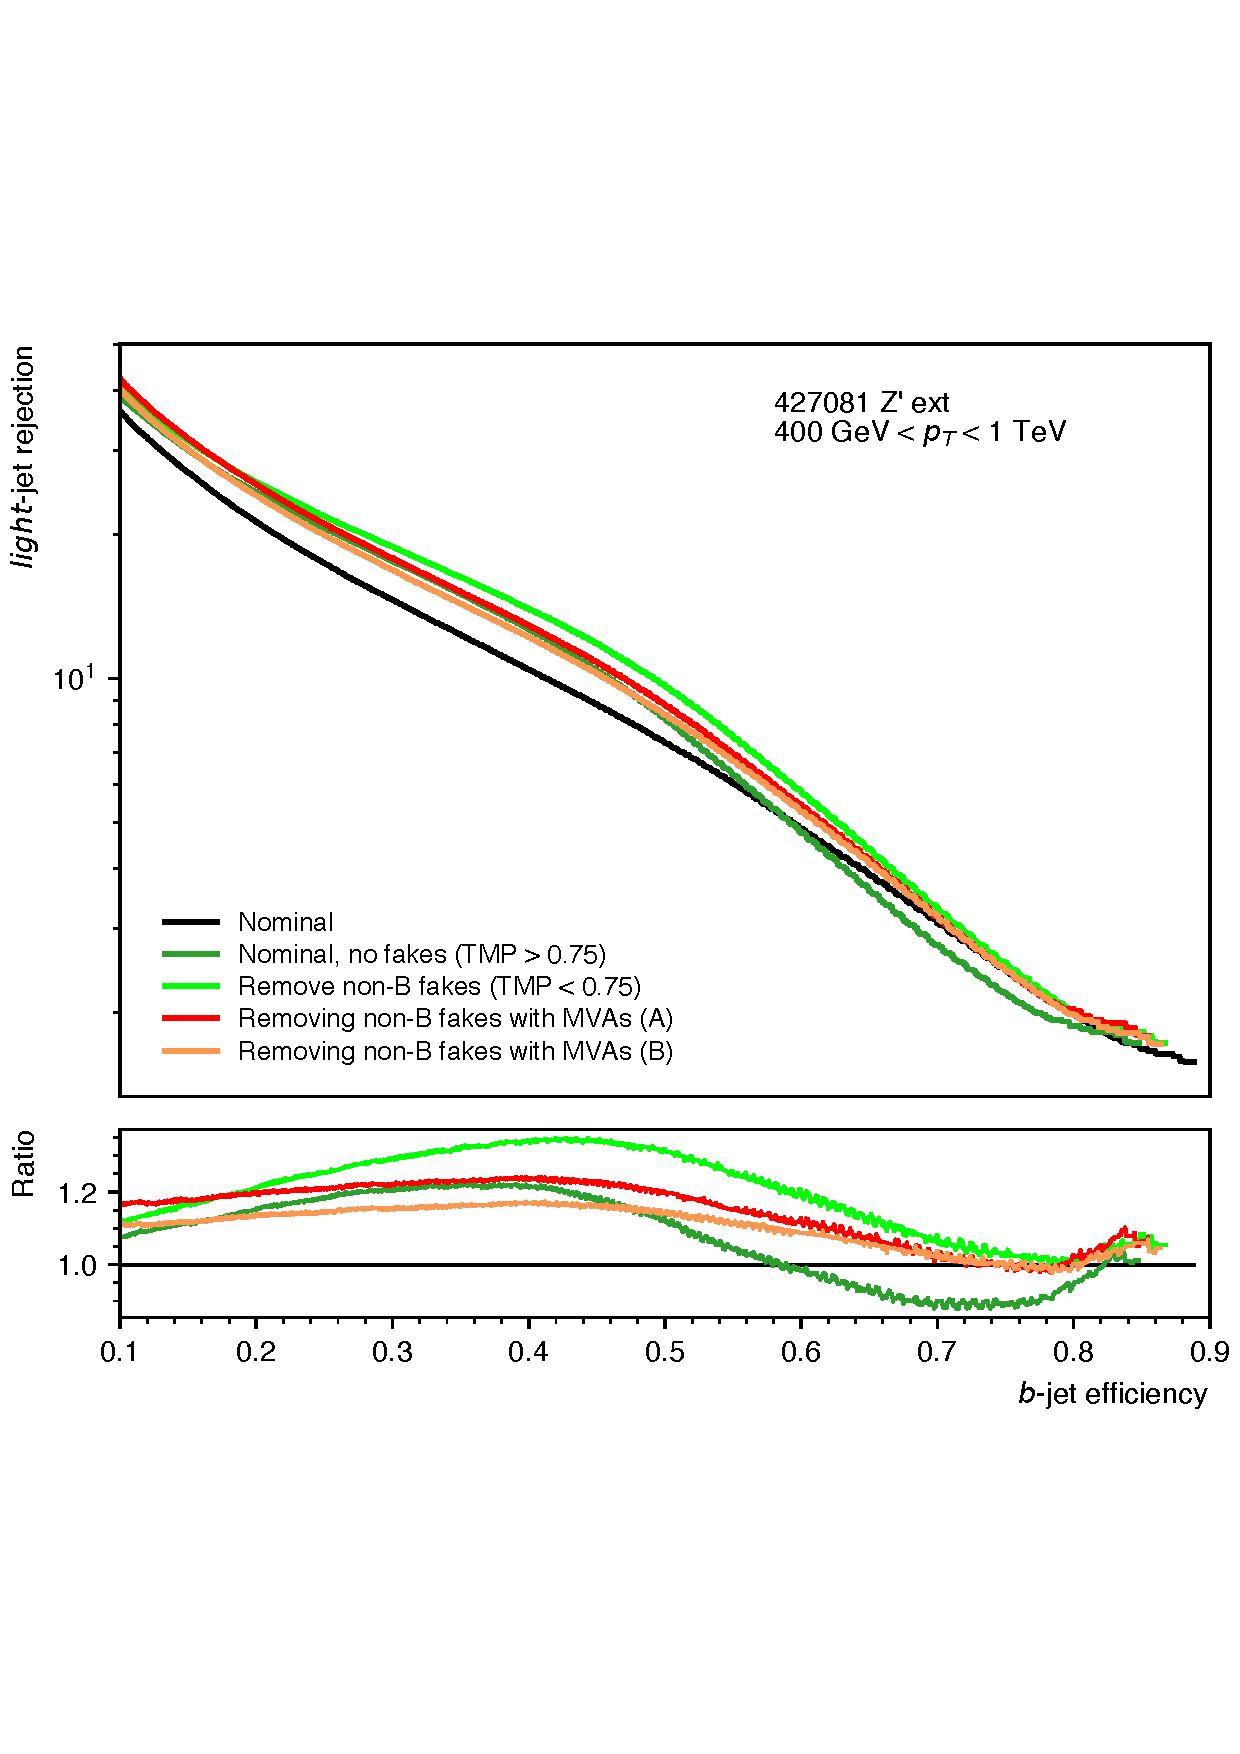
\includegraphics[width=\textwidth]{chapters/4.track_classifier/figs/zprime_jf_highpt.pdf}
%  \end{subfigure}
%  \caption{
    %The effect of applying the fake track identification algorithm alongside the \bhadron decay track identification on the jet tagging performance of JetFitter for jets with $\SI{250}{\GeV} < \pt < \SI{400}{\GeV}$ (left) and for jets with $\SI{400}{\GeV} < \pt < \SI{1}{\TeV}$ (right).
%    The nominal JetFitter \lrej (black) is compared to two working points of fake track removal, labelled ``A'' (red) and ``B'' (orange).
%    Removal of fake tracks based on truth information is shown by the green curves.
%  }
%  \label{fig:track_mva_jf}
%\end{figure}



\section{Conclusion}\label{sec:fake_track_mva_conclusion}

Fake tracks, which are prevalent in the core of high \pt jets, have an adverse impact on the performance of the low-level \btagging algorithms SV1 and JetFitter.
A ML tool to identify fake tracks has been developed.
The tool can be used to limit the number of fake tracks being input to the low-level tagging algorithms.
An advantage of the approach is that the continuous output of the model allows for the tuning of good and fake track identification efficiencies.
Since it was found that \bhadron decay tracks can also be poorly reconstructed and thus marked as fake, it was deemed necessary also to train a second algorithm to detect \bhadron decay tracks so that the removal of these tracks could be avoided.
Removing fake and non-$b$ decay tracks in this way was found to improve the \ljet mistagging rate of SV1 and JetFitter by up to \pct{20} at high transverse momentum.
The improvement achieved using the classification tools was generally comparable with that achieved when using the truth information to remove the fake tracks not from the decay of a \bhadron, demonstrating the efficacy of the approach.

\subsubsection{Future Work}
While removing tracks prior to their input to the low level tagging algorithms is shown here to be beneficial, a more performant alternative might be to keep these tracks but label them as being fake (for example using the output of the classification tool), and allow the tagging algorithms to take this into consideration.
This is not straightforward with manually optimised low-level taggers such as SV1 and JetFitter, but is possible with more advanced taggers as described in \cref{chap:gnn_tagger}.

Tools which identify the origin of a given track have other potential uses.
One application is to isolate a relatively pure sample of fake tracks which can be used to estimate the fake track rate in data, which would be useful for estimating the uncertainty on fake track modelling.
Another application is to use the \bhadron track identification tool to improve the track-to-jet association.
Both applications are currently under investigation within \ATLAS.

The approach here works on a track-by-track basis, but a more sophisticated approach would consider the correlations between the tracks inside a jet.
Also left for future work is to simultaneously train a single tool which discriminates between all the truth origins listed in \cref{tab:truth_origins}.
Such a tool would be useful as a general purpose track origin classifier.
An algorithm which takes both these aspects into consideration is discussed in \cref{chap:gnn_tagger}.
